% this file is called up by thesis.tex
% content in this file will be fed into the main document

%: ----------------------- name of chapter  -------------------------
\chapter{Modelli di movimento}\label{movimento} % top level followed by section, subsection


%: ----------------------- paths to graphics ------------------------

% change according to folder and file names
%\graphicspath{{2-Consorzi/images/}}


%: ----------------------- contents from here ------------------------
One important characteristic to achieve a good level of realism in DTN simulations is to simulate movement of nodes inside the simulated world. In Delay Tolerant Networks, movement of nodes is essential for the performance of the network, since end-to-end connectivity does not always exist and packets are delivered in a store and forward manner. For this reason is fundamental to simulate, with a good level of realism, movements behaviour of nodes inside the simulation.
\\

 Capturing movement accurately in the real usage scenarios is thus needed for a reliable assessment of a new protocol. Movement can be captured in simulations by either using real movement traces or synthetic traces generated by a movement model.

Uno degli aspetti più importante per garantire la realisticità di una simulazione riguarda il comportamento dei nodi, in particolare il loro movimento. Come è facile intuire, in una DTN i cambiamenti di posizione dei vari nodi influiscono pesantemente la connettività e quindi le prestazioni dell'intera rete. Proprio per questo motivo è fondamentale simulare il più realisticamente possibile il comportamento dei nodi all'interno della simulazione.


Il simulatore TheONE contiene al suo interno diversi modelli di movimento che possono essere assegnati ai vari gruppi di nodi. Presenterò ora un breve riassunto dei modelli a disposizione, soffermandomi in particolare su quello scelto per le simulazioni svolte, ossia il Working Day Movement Model (WDM)


\section{The map}
\label{mappaONE}
The map defines the space and routes in which the nodes can move inside the simulated world. The design of the map is an important part of the mobility model because it contains all the information of the locations of the houses, offices and meeting spots, as well as bus routes with bus stops. Since all the movement of the nodes is determined by activities with specific locations, the placement of these locations define how nodes are moving on a larger scale. Locations can be node group specific, i.e. some offices are used only by nodes in one group, nodes in different groups live in different houses locations, etc.. This makes it possible to create small districts within the map. In Fig. \ref{imgMappaABCD} is shown the default map included in the ONE simulator and used for our simulations and described in \cite{articoloWDM}.

\begin{figure}[htpb]
  \begin{center}
    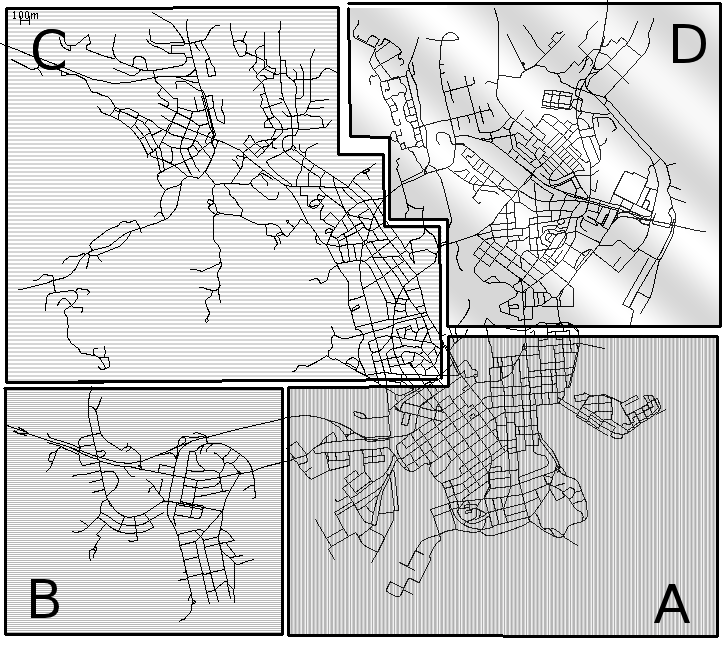
\includegraphics[scale=0.6]{figure/mappa_ABCD.png}
    \caption[Helsinky map]{The map of the Helsinki centre area used in our simulations}    
    \label{imgMappaABCD}
  \end{center}
\end{figure}

It is possible to see the four main district in which the map is divided. 
\\

In this implementation, every node group belongs to a district i.e. all nodes in one group will have their home location, office and meeting spot inside the related district. This is useful to limit node movement to small areas. Doing this we increased locality and it is not possible that nodes belonging to different groups (and so different districts) can meet each others. To decrease locality it is possible to spread houses, offices and meeting spots on the map, having nodes meeting easily.
\\

It is also possible to combine low and high locality: in Helsinki map used for our simulations there are four main districts, with different sizes, overlapped by other districts. This allows to have high locality but also some movement between districts, which corresponds to nodes coming to some district to work or meet friends, while others are leaving their district for similar reasons. Nodes moving between districts, not located next to each other, will have to pass through other districts. In Table \ref{tabellaDistrettiMappa} is shown distribution of nodes, offices and meeting spots in the districts of the map.

\begin{table}[h]
\begin{center}
\begin{tabular}{|l|c|c|c|}
\hline
\textbf{District} & \textbf{Nodes} & \textbf{Offices} & \textbf{Meeting spots}\\
\hline
\hline
\bfseries A & 150 & 30 & 4 \\
\hline
\bfseries B & 50 & 10 & 1 \\
\hline
\bfseries C & 100 & 20 & 2 \\
\hline
\bfseries D & 100 & 20 & 2 \\
\hline
\bfseries E (A + B) & 100 & 20 & 2 \\
\hline
\bfseries F (A + C) & 150 & 30 & 4 \\
\hline
\bfseries G (A + D) & 150 & 30 & 4 \\
\hline
\bfseries H (Whole map) & 200 & 40 & 5 \\
\hline
\end{tabular}
\end{center}
\caption[Helsinky map districts]{Table showing assignment of nodes, offices and meeting spots between districts in Helsinky map}    
\label{tabellaDistrettiMappa}
\end{table}


\section{Random Map-Based Movement}
Il modello più semplice fra quelli disponibili è il Random Map-Based Movement (MBM). I nodi che adottano questo modello si muovono in maniera casuale ma sempre seguendo le strade descritte dalla mappa della simulazione. Il risultato di questa modalità è un movimento troppo casuale per simulare accuratamente il comportamento umano per quanto riguarda la mobilità.

\section{Shortest Path Map-Based Movement}
Lo Shortest Path Map-Based Movement (SPMBM) è un modello leggermente più realistico rispetto a MBM. In questo modello i nodi scelgono casualmente un punto di destinazione all'interno della mappa e seguono la via più breve per raggiungerlo dalla posizione attuale, sempre seguendo le strade descritte dalla mappa della simulazione. Le destinazioni possono essere scelte in maniera completamente casuale o da un insieme di Punti di Interesse, in modo da simulare l'attrazione delle persone per luoghi come punti di ristoro, negozi o attrazioni turistiche.

\section{Routed Map-Based Movement}
Un modello che invece della casualità nel movimento utilizza dei percorsi predeterminati è il Routed Map-Based Movement (RMBM). I nodi che adottano questo modello si muovono lungo rotte predefinite, per tutta la durata della simulazione, rendendo RMBM utile per rappresentare degli spostamenti ripetitivi, come ad esempio quelli di autobus, tram o treni.

\section{Working Day Movement Model}
\label{descrWDM}
I modelli finora descritti sono senz'altro di semplice comprensione e realizzazione, oltre ad essere molto efficienti per quanto riguarda le prestazioni, ma non forniscono una realistica rappresentazione del movimento umano, soprattutto per quanto riguarda i valori di inter-contact e contact time.
\\
Un modello che genera dei valori più realistici per questi parametri, rappresentando più realisticamente quindi il movimento umano, è il Working Day Movement Model (WDM). Come il nome può fare intuire, questo modello simula gli spostamenti compiuti da una persona durante una tipica giornata lavorativa e in \cite{articoloWdm}, dove è descritto il modello, è evidenziato anche come i valori generati seguano realisticamente quelli trovati utilizzando dati di spostamento provenienti da tracce reali. 
\\
Una giornata simulata comprende le seguenti attività principali svolte dai vari nodi:
\begin{itemize}
\item dormire a casa
\item lavorare in ufficio
\item uscire alla sera con gli amici
\end{itemize}

Ovviamente le attività potrebbero cambiare enormemente a seconda dello stile di vita e del lavoro svolto dalle singole persone, ma queste tre attività sono le più comuni e possono essere associate alla tipica giornata di una gran quantità di persone.
La ripetitività giornaliera delle azioni e il fatto di svolgerle in luoghi comuni a più persone permette la formazione spontanea di comunità: persone che vivono e dormono nella stessa casa formeranno una famiglia, più persone che lavorano nello stesso ufficio agli stessi orari saranno colleghi di lavoro, mentre degli amici si possono trovare ad orari comuni alla sera per uscire assieme.
La creazione di queste comunità non viene mostrata da modelli più semplici quali RMBM o SPMBM.
\\

Per la simulazione delle attività giornaliere, WDM utilizza dei sottomodelli dedicati, oltre a dei sottomodelli preposti a simulare gli spostamenti fra un'attività e l'altra. Una persona si potrà quindi spostare a piedi, in auto o utilizzando i mezzi pubblici, a seconda della propria disponibilità e convenienza. Il fatto di muoversi da soli o in gruppo (prendendo lo stesso bus o camminando assieme la sera) permette di avere dei comportamenti eterogenei e quindi migliorare ulteriormente la realisticità degli spostamenti compiuti dai vari nodi.
\\

\subsection{Esempio di giornata}
Durante una tipica giornata il punto di partenza per ogni nodo è la propria abitazione. Ogni nodo ha un orario di sveglia assegnato, generato utilizzando una distribuzione normale con media pari a 0 e deviazione standard impostabile in fase di configurazione, che indica l'orario in cui la persona uscirà di casa. Il valore viene generato per ogni ad inizio simulazione, rimarrà lo stesso per tutti i giorni successivi e la differenza fra i valori di vari nodi sta ad indicare la differenza fra i diversi stili di vita nella vita reale (ad esempio una persona che impiega pochi minuti a prepararsi la mattina rispetto a chi impiega ore anche solo per fare colazione).
\\ 

Una volta usciti di casa, i vari nodi si dirigono al lavoro utilizzando l'auto (se disponibile) o a piedi oppure utilizzando i mezzi pubblici, a seconda di quale sia il metodo più conveniente. Conseguentemente alla scelta del mezzo di trasporto viene utilizzato il corrispondente sottomodello.
\\

Una volta raggiunto il luogo di lavoro, la persona ci resta per la durata della sua giornata lavorativa e quindi decide, con una determinata probabilità, se tornare direttamente a casa o spostarsi per un'attività serale. Anche in questo caso gli spostamenti vengono gestiti utilizzando i corrispondenti sottomodelli.


\subsection{Home Activity Submodel}
Ogni nodo ha una posizione impostata come Home Location, che viene utilizzata come punto di partenza alla mattina e punto di ritorno alla sera: una volta tornata a casa una persona si muove per una breve distanza e poi resta ferma fino all'orario di risveglio, la mattina successiva. Questo comportamento non è un errore, ma simula il fatto di lasciare il telefono su di un tavolo o in carica fino al momento di uscire nuovamente di casa, mentre la persona svolge le normali attività domestiche come mangiare, guardare la TV o dormire.

\subsection{Office Activity Submodel}
Il sottomodello relativo all'attività lavorativa è un modello bidimensionale che simula il comportamento di una persona all'interno di un ufficio, in cui è posizionata la propria scrivania e dalla quale ogni tanto si alza per partecipare ad una riunione, parlare con un collega o, perché no, per una pausa caffè. Durante tutti questi momenti, come è facile intuire, è possibile che il nodo entri in contatto con nodi relativi ad altri colleghi di lavoro.
\\

L'ufficio è descritto come un'unica stanza con pianta rettangolare, in cui l'unico punto di ingresso, la porta, è l'angolo in alto a sinistra e ogni persona che vi lavora ha una scrivania posizionata in un determinato punto. Non viene simulata la presenza di muri all'interno della stanza, che quindi verrà descritta come un luogo più grande del normale, in modo da simulare il tempo impiegato per superare ostacoli, nel movimento dalla scrivania ad una destinazione interna all'ufficio.
\\

Una volta entrato, l'impiegato si muove subito camminando verso la propria scrivania, dove rimane per un periodo di tempo casuale, generato utilizzando una distribuzione di Pareto. Passato questo tempo il nodo sceglie una destinazione casuale all'interno dell'ufficio, cammina fino a raggiungerla e quindi attende per un periodo di tempo casuale generato utilizzando la stessa distribuzione di Pareto prima di tornare alla propria scrivania. La ripetizione del movimento dalla scrivania ad una posizione casuale interna all'ufficio continua fino al termine della giornata lavorativa, che ha una durata impostabile in fase di configurazione.
\\

I parametri della distribuzione possono essere impostati per ogni gruppo di nodi, in modo da simulare diversi tipi di attività all'interno del luogo di lavoro, dall'insegnante che ogni ora si deve spostare in un'aula diversa, ad un commesso che non lascia mai la propria postazione per tutto l'orario lavorativo.


\subsection{Evening Activity Submodel}
Il sottomodello Evening Activity simula attività che possono essere svolte dopo lavoro, nel tardo pomeriggio - sera, come andare a fare shopping, in un bar o a mangiare in una pizzeria o ristorante. Tali attività vengono svolte in gruppo e con una probabilità configurabile, che determina se la persona torna o meno subito a casa dopo il lavoro.
\\

Al termine della giornata lavorativa, il nodo si sposta verso il proprio luogo d'incontro preferito, che è una posizione impostata all'inizio della simulazione. Una volta arrivato attende che lo raggiungano un numero di persone sufficientemente elevato per formare un gruppo e cominciare quindi l'attività. Il numero massimo e minimo di persone che possono formare un gruppo è configurabile e quando tutti i gruppi per un determinato punto di ritrovo sono al completo ne viene creato un altro.
\\

Una volta che tutti i componenti del gruppo legato all'attività sono arrivati, camminano assieme per una breve distanza verso una destinazione scelta casualmente e quindi si fermano per un tempo più lungo, generato casualmente all'interno di valori preimpostati. Una volta terminata questa pausa (finita la cena, lo shopping o la visione di un film al cinema), le varie persone si separano e tornano verso casa.

\subsection{Transport Activity Submodel}
Il Transport Activity Submodel è il sottomodello incaricato di gestire gli spostamenti dei nodi fra le diverse attività.
\\

All'inizio della simulazione ad ogni nodo viene assegnata un'auto con una probabilità configurabile. Le persone che la possiedono la utilizzeranno per tutti gli spostamenti, mentre chi ne è sprovvisto si muoverà a piedi o utilizzando un mezzo pubblico. L'eterogeneità di mezzi di trasporto utilizzati permette di simulare realisticamente i movimenti di diverse tipologie di persone ed inoltre ha impatto anche sul protocollo di routing utilizzato, in quanto nodi che si muovono utilizzando mezzi propri si sposteranno più velocemente, permettendo così il trasporto più rapido di pacchetti per lunghe distanze.
\\

A seconda del mezzo di trasporto utilizzato, quindi, il Transport Activity Submodel si rifà a tre sottomodelli distinti:
\\

\begin{description}
\item [Walking Submodel]: i nodi che non possiedono un'auto si muovono camminando lungo le strade ad una velocità costante, utilizzando l'algoritmo di Dijkstra per provare il percorso più breve dalla posizione corrente alla destinazione.
\item [Car Submodel]: i nodi che possiedono un'auto muovono più velocemente dei pedoni, durante le transizioni fra attività, ma si muovono come gli altri nodi all'interno di una singola attività. Non vengono considerati traffico e semafori durante la guida e ogni auto può portare una sola persona (il car sharing non ha ancora avuto successo nel mondo simulato).
\item [Bus Submodel]: nella città possono essere presenti più linee di trasporti pubblici (tram, autobus, funivie), ognuna delle quali viene percorsa da più mezzi ad orari predefiniti. Ogni mezzo pubblico può trasportare più persone.
\end{description}


Ogni persona che non possiede un'auto conosce una linea di mezzi pubblici e può utilizzare qualunque mezzo appartenente a quella linea. Il fatto di prendere il mezzo pubblico o di camminare dipende da un confronto di distanze euclidee: la distanza fra il luogo di partenza e quello di destinazione oppure quella fra il luogo di partenza e la fermata più vicina sommata alla distanza fra la destinazione e la fermata più vicina alla destinazione. Nel caso sia minore la prima allora il nodo camminerà fino alla destinazione, altrimenti utilizzerà i mezzi pubblici. Per fare ciò camminerà fino alla fermata più vicina, utilizzando il Walking Submodel, attenderà il primo mezzo che passerà per quella linea nella direzione corretta, utilizzerà il Bus Submodel fino alla fermata più vicina alla destinazione e quindi tornerà ad utilizzare il Walking Submodel camminando fino al punto di arrivo.
 
% ---------------------------------------------------------------------------
%: ----------------------- end of thesis sub-document ------------------------
% ---------------------------------------------------------------------------

